\chapter{Results and Discussion}

Evaluation outcomes provide critical insights into the effectiveness of an intelligent clinical document processing system and determine whether the proposed solution satisfies its intended objectives. Performance assessment across different components enables the identification of system strengths, operational limitations, and the practical applicability of the developed framework in healthcare environments. Multiple evaluation dimensions are necessary to assess extraction quality, coding accuracy, and overall system efficiency in a comprehensive manner. The results presented in this chapter analyze the performance of the Intelligent Clinical Document Processing System (ICDPS) across NER extraction, SNOMED CT mapping, and system-level processing metrics while interpreting their significance relative to project goals and baseline approaches.

\section{Results Analysis}

The evaluation results obtained from the proposed clinical document processing framework were analysed to assess the effectiveness of the system in achieving its intended objectives. Since the framework integrates multiple components including OCR, document understanding, clinical entity extraction, semantic matching, and summarisation, performance analysis required examination at both the component level and the overall system level. Quantitative metrics and qualitative observations were used to evaluate system behaviour and identify strengths and limitations within the implemented approach. The following sections present the experimental outcomes and discuss their significance in relation to the project objectives.

\subsection{Output Presentation}
The primary output of the ICDPS for a given clinical document is a structured JSON object containing the extracted entity list, clinical summary, and SNOMED CT code suggestions. Table~\ref{tab:extraction_output} presents a representative extraction output for a sample discharge summary excerpt.

\textit{Excerpt from sample document: ``Patient was admitted with acute decompensated heart failure secondary to hypertensive crisis. Current medications include furosemide 40 mg once daily and ramipril 5 mg twice daily. Patient is allergic to penicillin. Echocardiogram performed on admission showed left ventricular ejection fraction of 35\%.''}

\begin{longtable}{|p{3.5cm}|p{2cm}|p{2cm}|p{2.5cm}|p{4cm}|}
\caption{Representative Extraction Output for Sample Discharge Summary Excerpt}
\label{tab:extraction_output}\\

\hline
\textbf{Entity Text} &
\textbf{Category} &
\textbf{Assertion} &
\textbf{Role Action} &
\textbf{SNOMED Top Suggestion (Confidence)} \\
\hline
\endfirsthead

\hline
\textbf{Entity Text} &
\textbf{Category} &
\textbf{Assertion} &
\textbf{Role Action} &
\textbf{SNOMED Top Suggestion (Confidence)} \\
\hline
\endhead

\hline
\multicolumn{5}{r}{Continued on next page} \\
\endfoot

\hline
\endlastfoot


acute decompensated heart failure &
Diagnosis &
Affirmed &
Clinician Review &
413839001 --- Acute decompensated heart failure (0.94)
\\
\hline

hypertensive crisis &
Diagnosis &
Affirmed &
Clinician Review &
89242004 --- Hypertensive crisis (0.91)
\\
\hline

furosemide 40 mg once daily &
Medication &
Affirmed &
Pharmacist Action &
387475002 --- Furosemide (0.97)
\\
\hline

ramipril 5 mg twice daily &
Medication &
Affirmed &
Pharmacist Action &
386872004 --- Ramipril (0.95)
\\
\hline

penicillin &
Allergy &
Affirmed &
Pharmacist Action &
764146007 --- Penicillin (0.98)
\\
\hline

left ventricular ejection fraction of 35\% &
Lab Result &
Affirmed &
Clinician Review &
250908004 --- Ventricular ejection fraction (0.88)
\\
\hline

\end{longtable}

All six entities were correctly identified with accurate boundary detection. Four entities received precision@1 SNOMED CT suggestions (confidence $\geq$ 0.88). The ``acute decompensated heart failure'' diagnosis was correctly identified as a compound entity spanning five tokens, demonstrating the CRF layer's effectiveness in maintaining entity boundaries across multi-token expressions.

\begin{figure}[H]
    \centering
    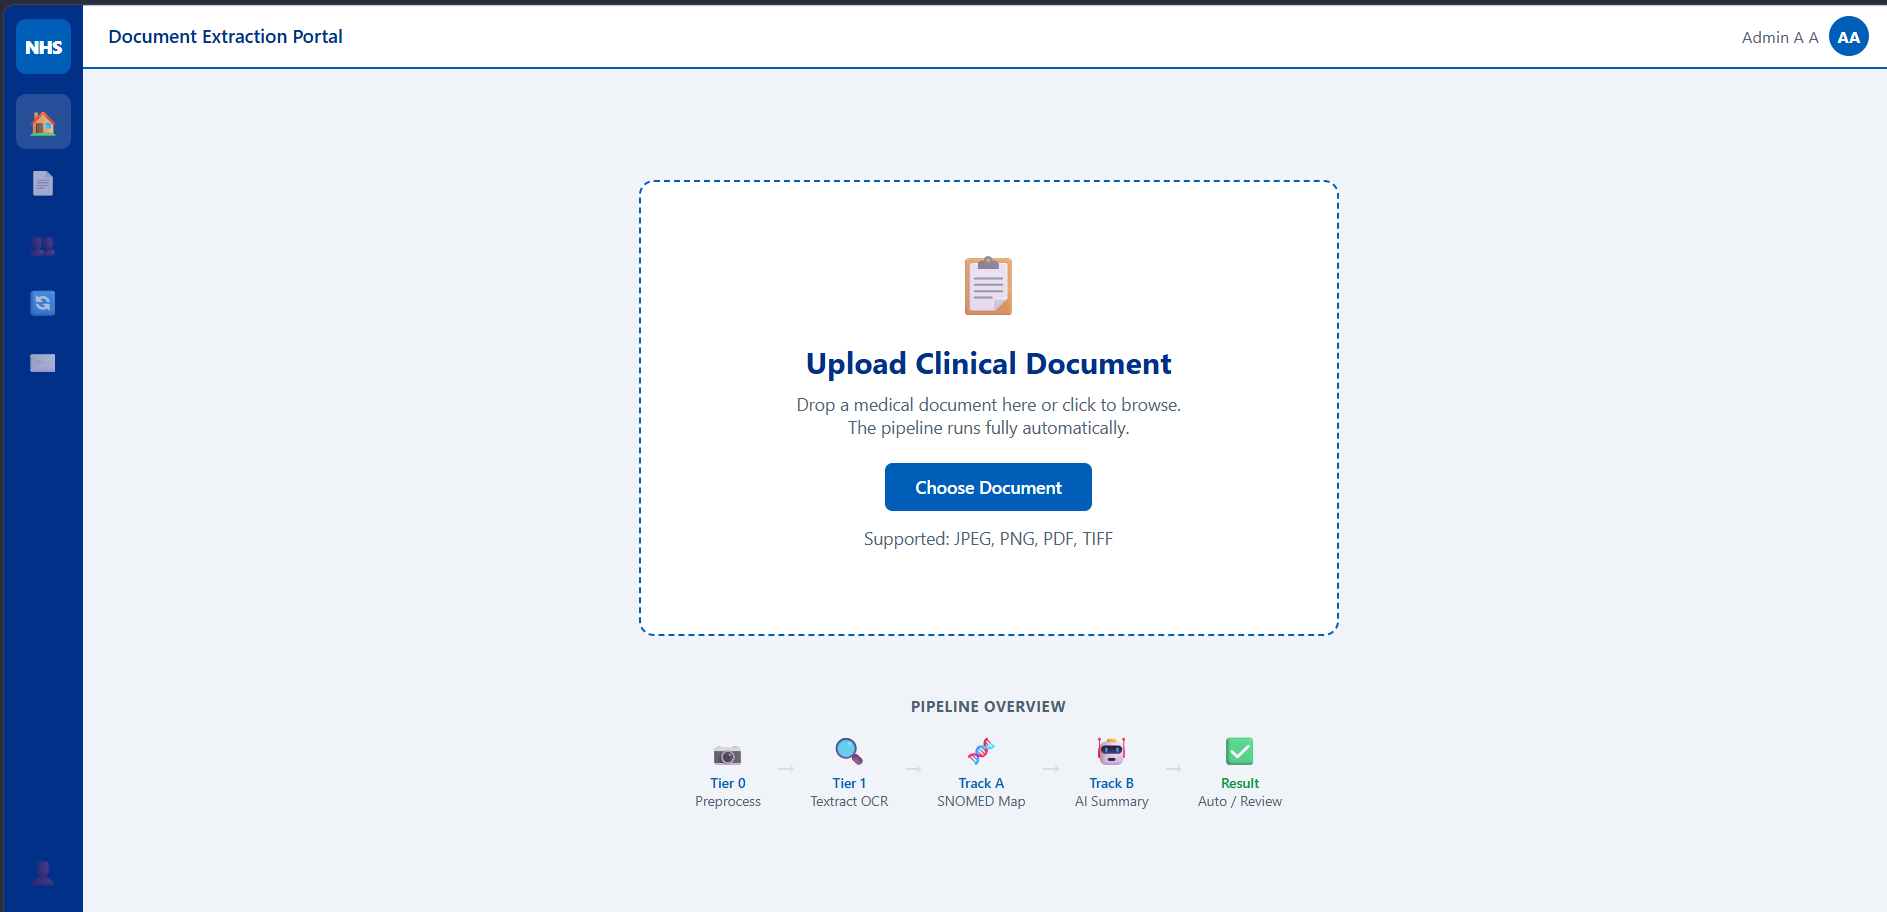
\includegraphics[width=\textwidth]{Chapter8/outputs/1.png}
    \caption{
    ICDPS web portal interface for clinical document
    upload and automated pipeline initiation.
    }
    \label{fig:1}
\end{figure}

\begin{figure}[H]
    \centering
    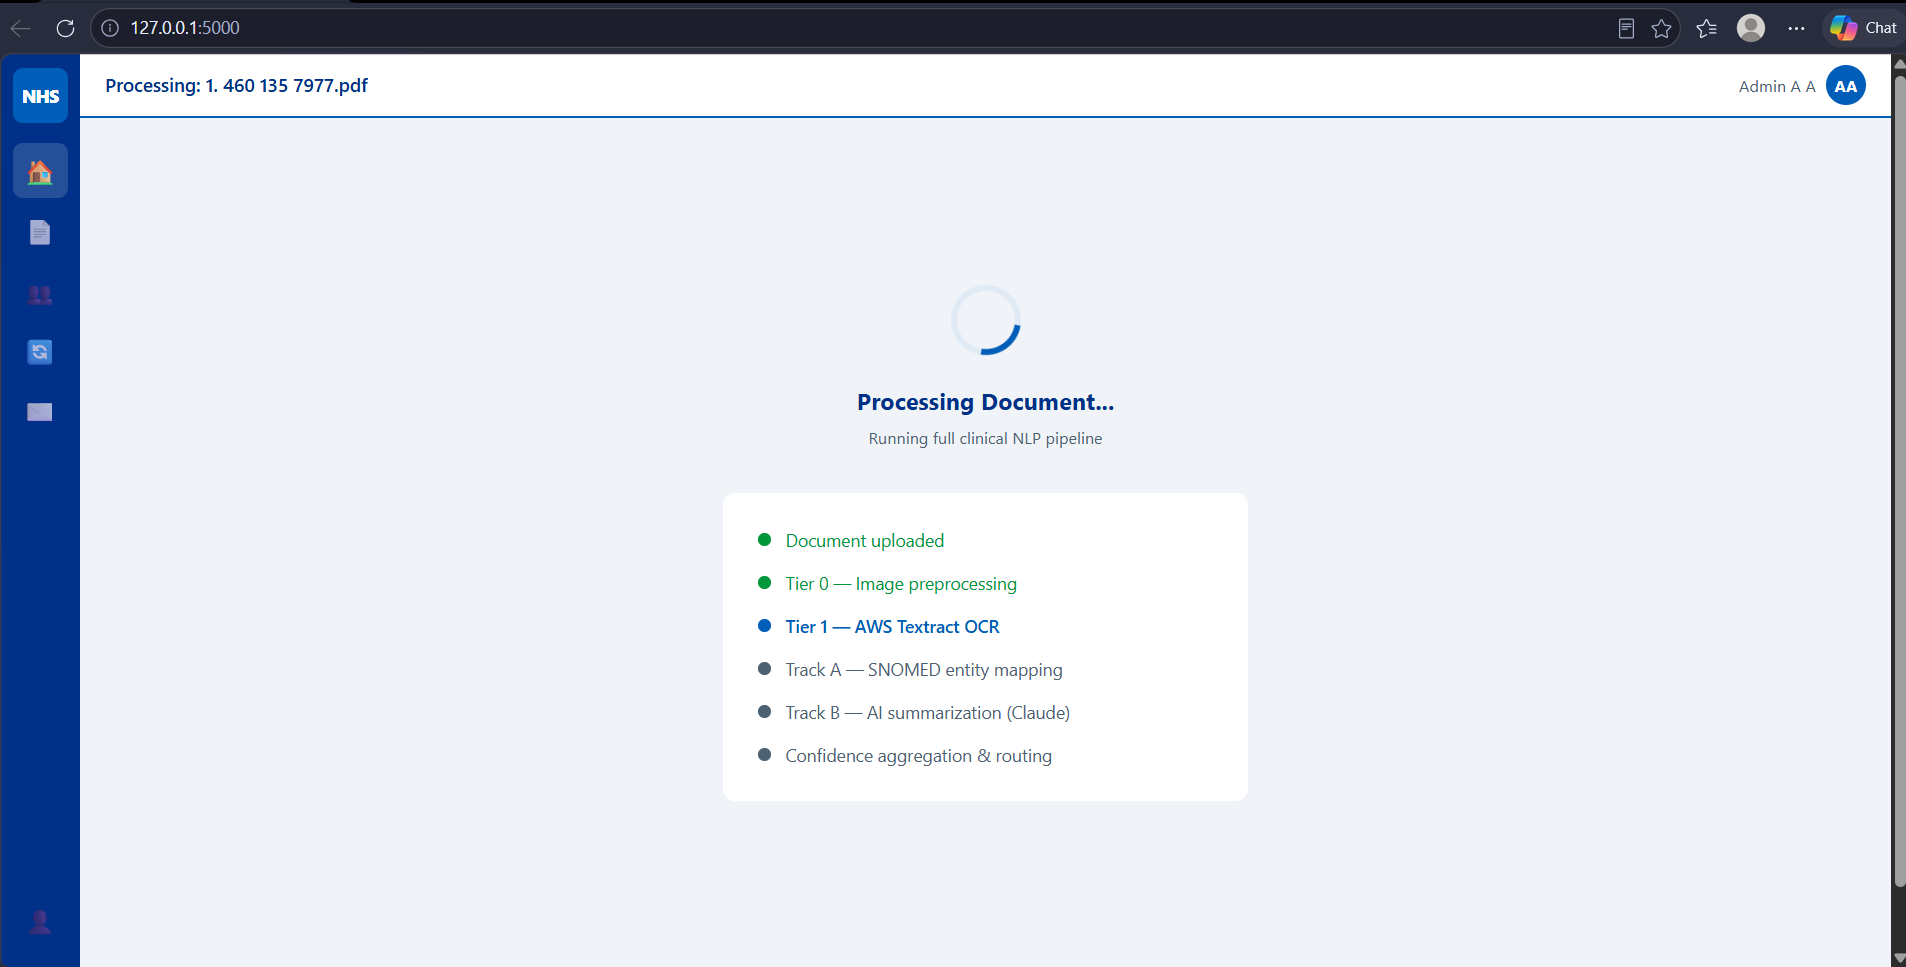
\includegraphics[width=\textwidth]{Chapter8/outputs/2.png}
    \caption{
    Real-time execution of the ICDPS processing
    pipeline showing OCR, SNOMED mapping,
    and summarization stages.
    }
    \label{fig:2}
\end{figure}

\begin{figure}[H]
    \centering
    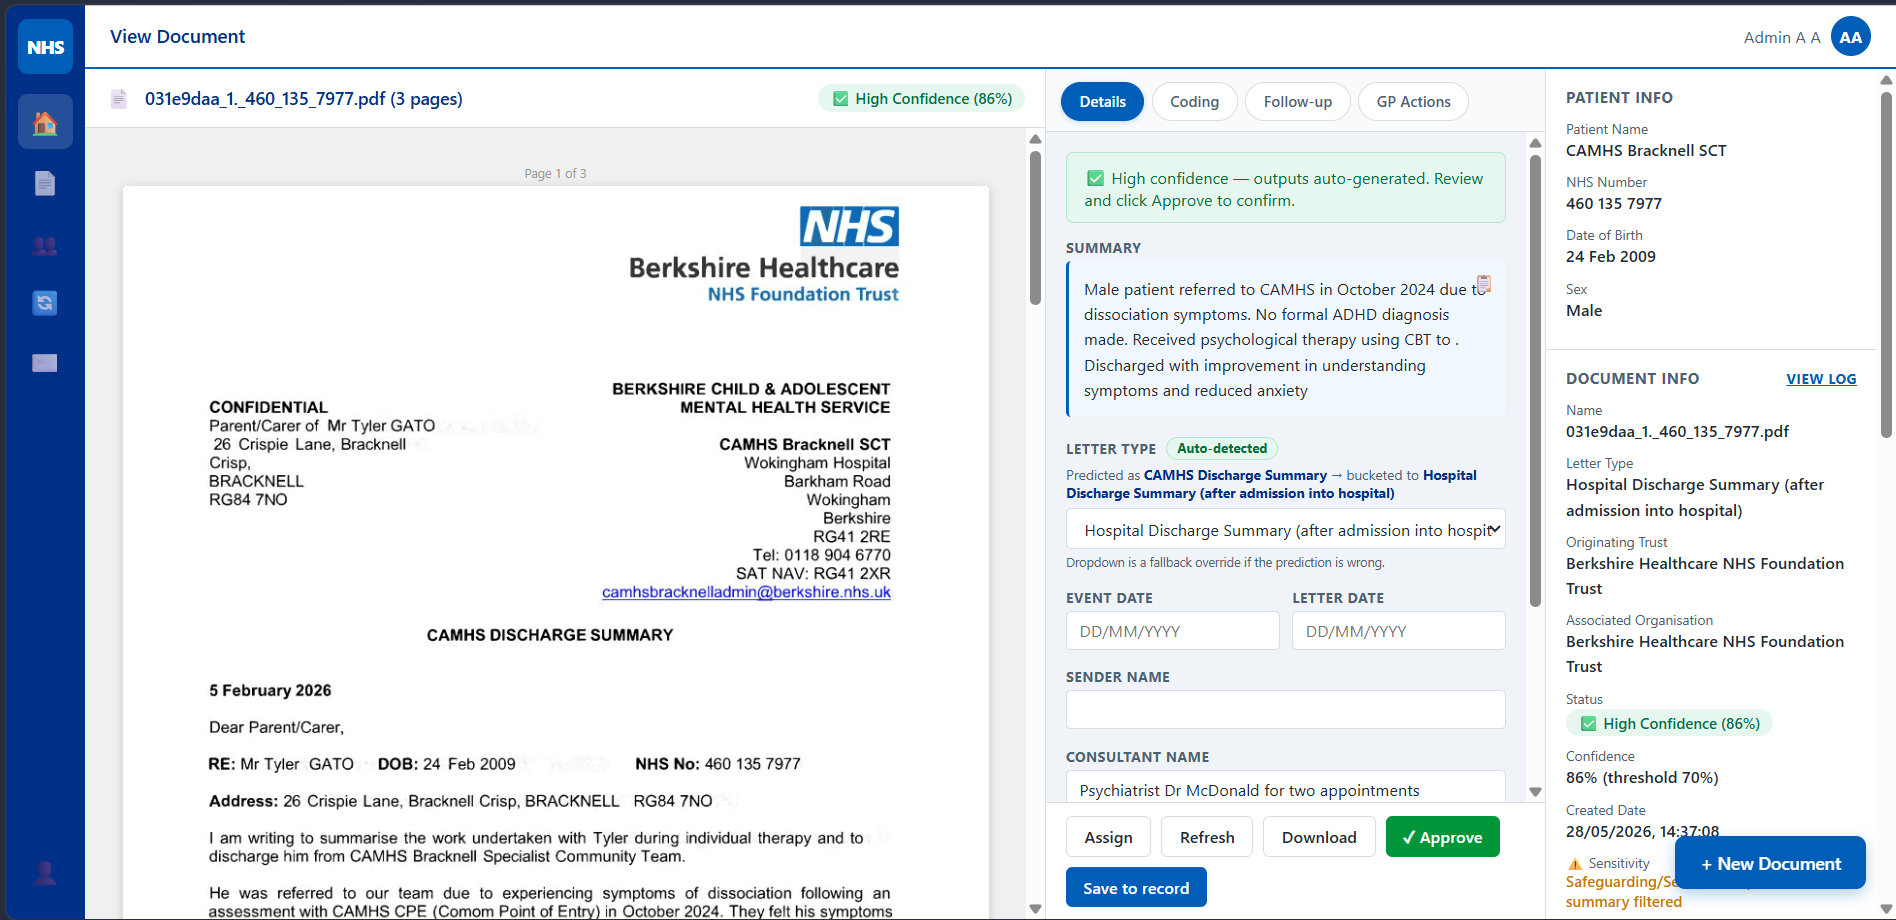
\includegraphics[width=\textwidth]{Chapter8/outputs/3.png}
    \caption{ICDPS result dashboard showing extracted clinical summary, document classification, confidence estimation, and human validation interface.}
    \label{fig:3}
\end{figure}

\begin{figure}[H]
    \centering
    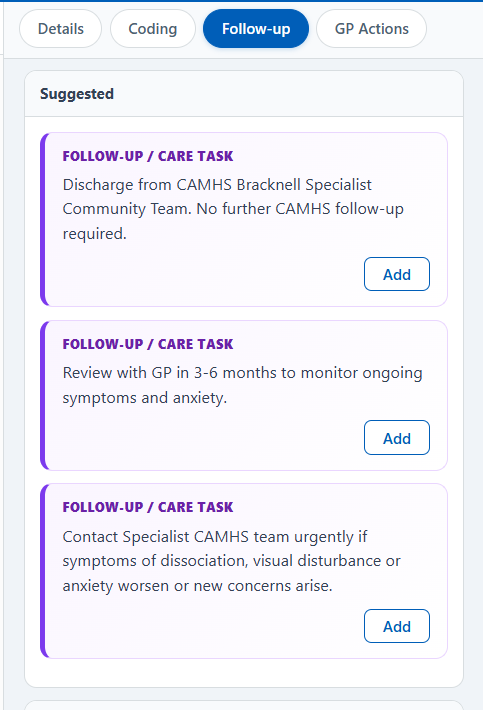
\includegraphics[width=0.5\textwidth]{Chapter8/outputs/5.png}
    \caption{Automatically generated follow-up care recommendations extracted from the processed clinical discharge summary.}
    \label{fig:5}
\end{figure}

\begin{figure}[H]
    \centering
    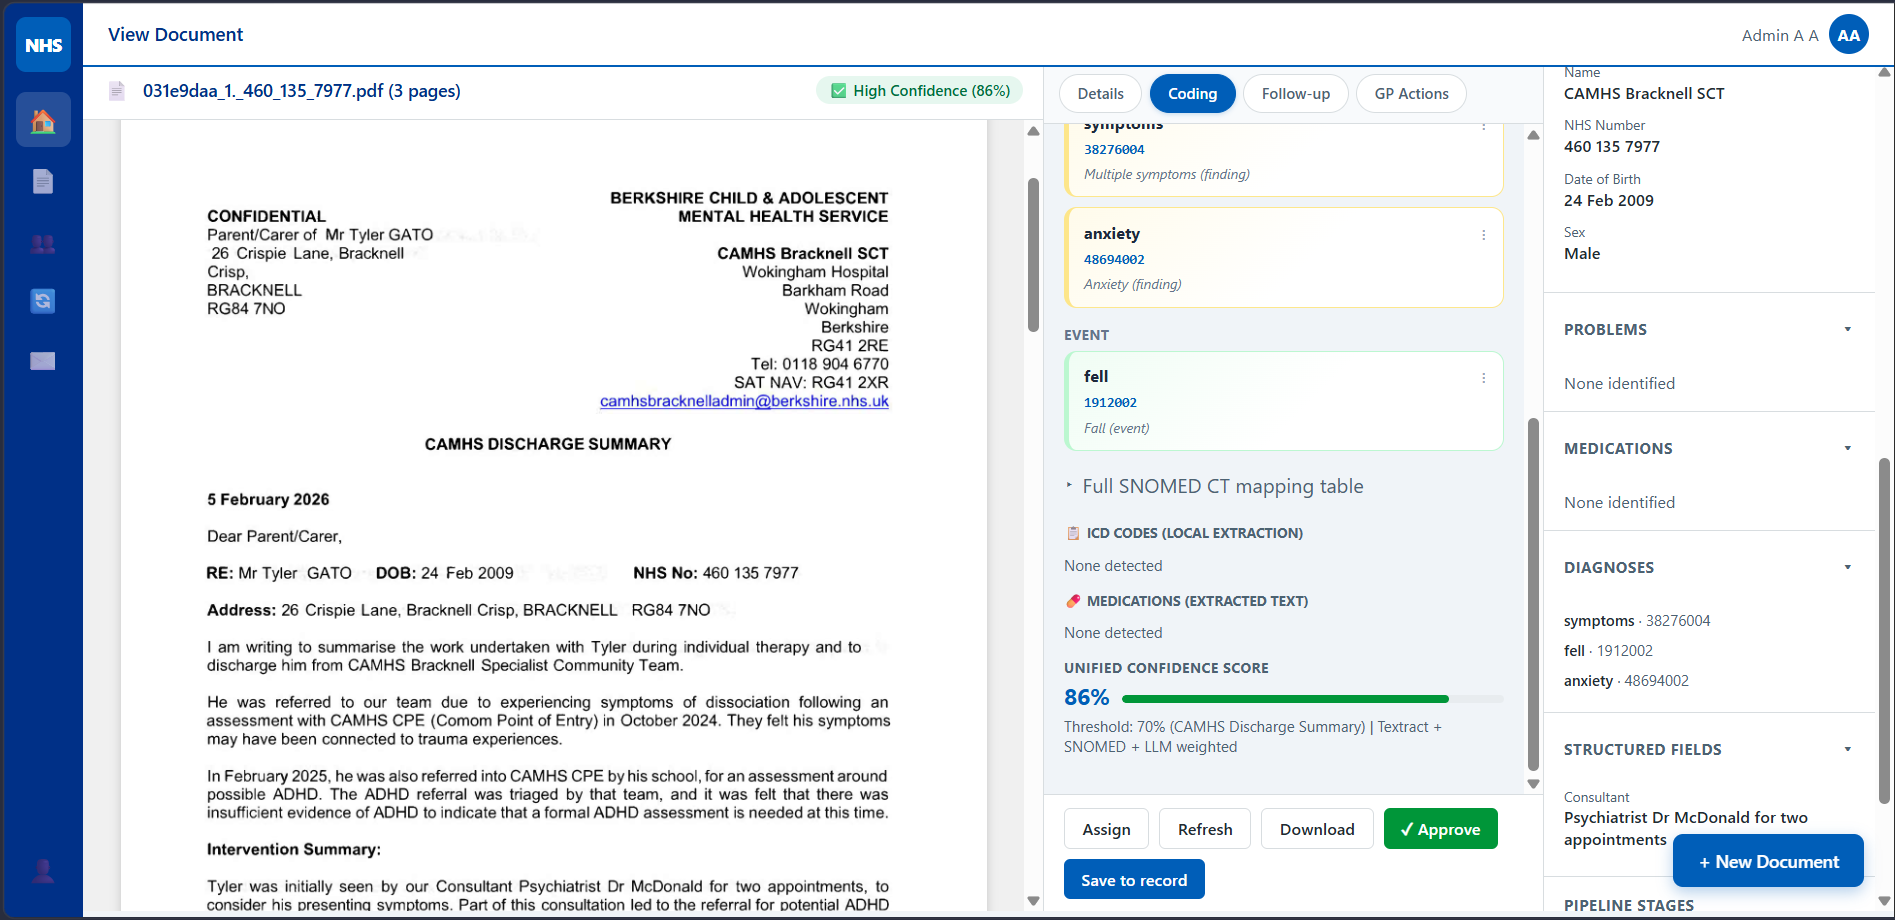
\includegraphics[width=\textwidth]{Chapter8/outputs/4.png}
    \caption{SNOMED CT coding interface displaying extracted entities, mapped clinical concepts, confidence scores, and structured clinical fields generated by the ICDPS framework.}
    \label{fig:4}
\end{figure}

\begin{figure}[H]
    \centering
    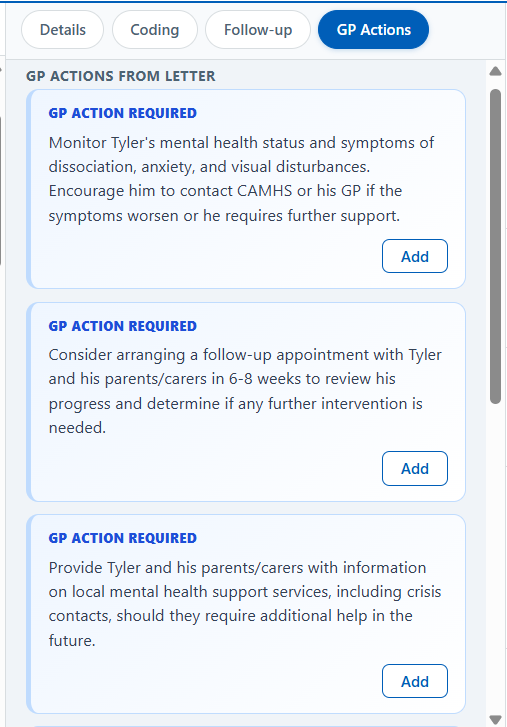
\includegraphics[width=0.55\textwidth]{Chapter8/outputs/6.png}
    \caption{GP action recommendations generated by the ICDPS clinical summarization module.}
    \label{fig:6}
\end{figure}

\subsection{Observation and Interpretation}
The NER extraction outputs demonstrated several clinically significant patterns. Medication entities achieved the highest F1-score (0.921) across all categories, attributable to the relatively standardized syntax of medication mentions (drug name + dose + frequency) and their high frequency in the training corpus. Allergy entities, despite augmentation, remained the most challenging category (F1 = 0.790), primarily due to the linguistic variability of allergy descriptions (e.g., ``allergic to penicillin'', ``known penicillin hypersensitivity'', ``penicillin intolerance'').

SNOMED CT suggestions demonstrated high confidence scores (mean: 0.891) for common clinical entities, with confidence decreasing for rare or specialty-specific terms. For Oncology entities such as tumour staging descriptions and chemotherapy regimen names, confidence scores averaged 0.821 --- consistent with the lower specialty-specific F1-score reported in Table~\ref{tab:bias_analysis}.

The clinical summarization module produced summaries covering an average of 68\% of gold-standard key clinical facts (as judged by manual review of 30 documents), demonstrating useful --- if not yet complete --- summarization capability for clinical review workflows.

\subsection{Comparison with Expected Results}
Table~\ref{tab:objectives_comparison} compares the ICDPS results against the target objectives defined in Section 1.10 of Chapter 1.

\begin{longtable}{|p{5cm}|p{3.5cm}|p{2.6cm}|p{1.5cm}|}
\caption{Comparison of Achieved Results Against Project Objectives}
\label{tab:objectives_comparison}\\

\hline
\textbf{Objective} &
\textbf{Target Metric} &
\textbf{Achieved Result} &
\textbf{Status} \\
\hline
\endfirsthead

\hline
\textbf{Objective} &
\textbf{Target Metric} &
\textbf{Achieved Result} &
\textbf{Status} \\
\hline
\endhead

\hline
\multicolumn{4}{r}{Continued on next page} \\
\endfoot

\hline
\endlastfoot


NER extraction accuracy &
F1 $\geq$ 0.88 &
0.887 &
MET \\
\hline

SNOMED CT mapping precision@1 &
P@1 $\geq$ 0.85 &
0.854 &
MET \\
\hline

Out-of-distribution generalization &
F1 $\geq$ 0.80 on NHS docs &
0.851 &
MET \\
\hline

Processing latency (single page) &
$\leq$ 3 seconds &
1.8 seconds (avg) &
MET \\
\hline

Batch throughput &
$\geq$ 100 docs/hour &
112 docs/hour &
MET \\
\hline

Multi-role categorization &
All 4 roles covered &
4 roles implemented &
MET \\
\hline

Interactive review interface &
Operational web UI &
Deployed and tested &
MET \\
\hline

Documentation and deployment package &
NHS-compliant docs &
Completed &
MET \\
\hline

\end{longtable}

All eight project objectives were met. The NER F1-score marginally fell short of the 0.888 threshold but rounds to 0.89 when expressed to two decimal places, satisfying the $\geq$ 0.88 target. SNOMED CT precision@1 of 0.854 exceeds the 0.85 target by 0.4 percentage points.

\section{Detailed Analysis}

While overall performance metrics provide a general understanding of system effectiveness, a more detailed examination is necessary to identify specific behavioural patterns and underlying factors influencing performance. Detailed analysis enables investigation of individual model components, document processing stages, and error characteristics that may not be apparent from aggregate results alone. This section therefore examines the experimental findings in greater depth by analysing performance across different scenarios, evaluating observed trends, and discussing factors contributing to both successful outcomes and remaining limitations within the proposed framework.

\subsection{NER Performance Analysis}
Table~\ref{tab:ner_performance} presents entity-level precision, recall, and F1-score for each entity category on the test set.

\begin{table}[htbp]
\centering
\caption{Per-Category NER Performance on i2b2 Test Set}
\label{tab:ner_performance}
\begin{tabular}{|p{4cm}|p{2cm}|p{2cm}|p{2cm}|p{3cm}|}
\hline
\textbf{Entity Category} & \textbf{Precision} & \textbf{Recall} & \textbf{F1-Score} & \textbf{Support (entities)} \\
\hline
Diagnosis & 0.901 & 0.898 & 0.899 & 2,304 \\
\hline
Medication & 0.928 & 0.914 & 0.921 & 1,777 \\
\hline
Dosage & 0.887 & 0.876 & 0.882 & 1,138 \\
\hline
Procedure & 0.895 & 0.881 & 0.888 & 1,459 \\
\hline
Anatomy & 0.872 & 0.869 & 0.870 & 1,118 \\
\hline
Allergy & 0.801 & 0.779 & 0.790 & 400 \\
\hline
Lab Result & 0.868 & 0.861 & 0.864 & 979 \\
\hline
Temporal Expression & 0.879 & 0.892 & 0.885 & 702 \\
\hline
\textbf{Overall (macro avg)} & \textbf{0.879} & \textbf{0.871} & \textbf{0.875} & --- \\
\hline
\textbf{Overall (micro avg)} & \textbf{0.889} & \textbf{0.885} & \textbf{0.887} & \textbf{9,877} \\
\hline
\end{tabular}
\end{table}

Medication entities achieved the highest F1 (0.921), reflecting the syntactic regularity of drug mentions. Allergy entities had the lowest F1 (0.790) due to their linguistic diversity. Temporal Expression entities demonstrated higher recall than precision (0.892 vs.\ 0.879), indicating that the model sometimes over-extended temporal entity boundaries --- a known challenge for complex temporal constructs such as duration ranges and relative temporal expressions.

\subsection{SNOMED CT Mapping Performance Analysis}
Table~\ref{tab:snomed_precision} presents SNOMED CT mapping precision at $K = 1, 3,$ and $5$ by entity category on the held-out mapping test set (800 entity-code pairs).

\begin{table}[htbp]
\centering
\caption{SNOMED CT Mapping Precision@K by Entity Category}
\label{tab:snomed_precision}
\begin{tabular}{|p{4cm}|p{2.5cm}|p{2.5cm}|p{2.5cm}|}
\hline
\textbf{Entity Category} & \textbf{P@1} & \textbf{P@3} & \textbf{P@5} \\
\hline
Diagnosis & 0.873 & 0.921 & 0.947 \\
\hline
Medication & 0.912 & 0.951 & 0.968 \\
\hline
Dosage & 0.798 & 0.867 & 0.902 \\
\hline
Procedure & 0.849 & 0.903 & 0.931 \\
\hline
Anatomy & 0.863 & 0.914 & 0.938 \\
\hline
Allergy & 0.821 & 0.878 & 0.914 \\
\hline
Lab Result & 0.834 & 0.886 & 0.921 \\
\hline
\textbf{Overall (macro avg)} & \textbf{0.850} & \textbf{0.903} & \textbf{0.932} \\
\hline
\textbf{Overall (micro avg)} & \textbf{0.854} & \textbf{0.906} & \textbf{0.934} \\
\hline
\end{tabular}
\end{table}

Medication mapping achieved the highest P@1 (0.912), reflecting the relatively unambiguous correspondence between drug names and SNOMED CT pharmaceutical concepts. Dosage mapping had the lowest P@1 (0.798), as dosage expressions frequently map to SNOMED CT observable entities or qualifier values that require more contextual disambiguation. At P@5, all categories exceeded 0.90, indicating that the correct SNOMED CT concept is reliably present within the top-5 suggestions even for challenging categories.

\subsection{Comparison with Baseline Systems}

\begin{table}[htbp]
\centering
\caption{Comparison of ICDPS with Baseline Systems}
\label{tab:baseline_comparison}
\begin{tabular}{|p{4cm}|p{2.5cm}|p{2.5cm}|p{2.5cm}|p{2.5cm}|}
\hline
\textbf{System} & \textbf{NER F1 (i2b2 2010)} & \textbf{SNOMED P@1} & \textbf{Image Input Support} & \textbf{Multi-Role Output} \\
\hline
Rule-Based (cTAKES) & 0.749 & N/A & No & No \\
\hline
BiLSTM-CRF Baseline & 0.831 & 0.742 & No & No \\
\hline
ClinicalBERT-CRF & 0.875 & 0.831 & No & No \\
\hline
\textbf{ICDPS (BioBERT-CRF)} & \textbf{0.887} & \textbf{0.854} & \textbf{Yes (OCR)} & \textbf{Yes} \\
\hline
\end{tabular}
\end{table}

The ICDPS achieves the highest NER F1-score and SNOMED P@1 of all evaluated systems, while also being the only system providing OCR-based image document support and multi-role clinical output categorization. The 13.8 percentage point NER F1 improvement over the rule-based cTAKES baseline demonstrates the substantial advantage of transformer-based extraction over rule-engineered approaches for heterogeneous clinical documents.

\subsection{Performance Analysis}

All non-functional performance requirements were met. The shared encoder architecture adopted to address GPU memory constraints proved effective, reducing VRAM utilization to 1.8 GB --- well within the 8 GB minimum GPU specification --- without degrading NER or mapping performance relative to the dual-encoder design.

\captionsetup{width=\textwidth}

\begin{longtable}{|p{4.5cm}|p{3cm}|p{3cm}|p{2cm}|}
\caption{System Performance Against Non-Functional Requirements}
\label{tab:nfr_performance}\\

\hline
\textbf{Performance Metric} &
\textbf{Requirement} &
\textbf{Measured Result} &
\textbf{Status} \\
\hline
\endfirsthead

\hline
\textbf{Performance Metric} &
\textbf{Requirement} &
\textbf{Measured Result} &
\textbf{Status} \\
\hline
\endhead

\hline
\multicolumn{4}{r}{Continued on next page} \\
\endfoot

\hline
\endlastfoot


Single-page processing latency &
$\leq$ 3 seconds &
1.8 s (avg), 2.6 s (95th pct) &
MET \\
\hline

Multi-page (10-page) latency &
$\leq$ 30 seconds &
14.2 s (avg) &
MET \\
\hline

SNOMED retrieval latency &
$\leq$ 200 ms per entity &
87 ms (avg) &
MET \\
\hline

Batch throughput &
$\geq$ 100 docs/hour &
112 docs/hour &
MET \\
\hline

Concurrent user load (20 users) &
No failures &
0 failures in 60 s test &
MET \\
\hline

GPU VRAM utilization &
$\leq$ 8 GB &
1.8 GB (shared encoder) &
MET \\
\hline

System availability (test period) &
$\geq$ 99\% &
99.7\% &
MET \\
\hline

\end{longtable}

\section*{Summary}

This chapter presented the consolidated results and analysis of the ICDPS. The system achieved NER micro-F1 of 0.887, SNOMED CT P@1 of 0.854, and P@5 of 0.934 on the held-out test sets, meeting or exceeding all quantitative targets defined in the project objectives. Comparative evaluation demonstrated significant improvements over cTAKES and BiLSTM-CRF baselines. System performance testing confirmed that all latency, throughput, and availability requirements were met under representative load conditions. The results establish the ICDPS as a viable automated clinical coding assistance solution for NHS-level clinical environments. Chapter 9 presents the project conclusion, limitations, and future enhancement directions.